\documentclass[11pt]{article}
\usepackage{geometry}                
\geometry{letterpaper}                   

\usepackage{graphicx}
\usepackage{amssymb}
\usepackage{epstopdf}
\usepackage{natbib}
\usepackage{amssymb, amsmath}
\usepackage{hyperref}
\DeclareGraphicsRule{.tif}{png}{.png}{`convert #1 `dirname #1`/`basename #1 .tif`.png}

%\title{The Swiss Train Network}
%\author{Mario Vontobel, Elias Rieder}
%\date{date} 

\begin{document}



\thispagestyle{empty}

\begin{center}
\includegraphics[width=5cm]{ETHlogo.eps}

\bigskip


\bigskip


\bigskip


\LARGE{ 	Lecture with Computer Exercises:\\ }
\LARGE{ Modelling and Simulating Social Systems with MATLAB\\}

\bigskip

\bigskip

\small{Project Report}\\

\bigskip

\bigskip

\bigskip

\bigskip


\begin{tabular}{|c|}
\hline
\\
\textbf{\LARGE{The Swiss Train Network}}\\
\\
\hline
\end{tabular}
\bigskip

\bigskip

\bigskip

\LARGE{Mario Vontobel \& Elias Rieder}



\bigskip

\bigskip

\bigskip

\bigskip

\bigskip

\bigskip

\bigskip

\bigskip

Zurich\\
Dec 2014\\

\end{center}



\newpage

%%%%%%%%%%%%%%%%%%%%%%%%%%%%%%%%%%%%%%%%%%%%%%%%%

\newpage
\section*{Agreement for free-download}
\bigskip


\bigskip


\large We hereby agree to make our source code for this project freely available for download from the web pages of the SOMS chair. Furthermore, we assure that all source code is written by ourselves and is not violating any copyright restrictions.

\begin{center}

\bigskip


\bigskip


\begin{tabular}{@{}p{3.3cm}@{}p{6cm}@{}@{}p{6cm}@{}}
\begin{minipage}{3cm}

\end{minipage}
&
\begin{minipage}{6cm}
\vspace{2mm} \large Mario Vontobel

 \vspace{\baselineskip}

\end{minipage}
&
\begin{minipage}{6cm}

\large Elias Rieder

\end{minipage}
\end{tabular}


\end{center}
\newpage

%%%%%%%%%%%%%%%%%%%%%%%%%%%%%%%%%%%%%%%



% IMPORTANT
% you MUST include the ETH declaration of originality here; it is available for download on the course website or at http://www.ethz.ch/faculty/exams/plagiarism/index_EN; it can be printed as pdf and should be filled out in handwriting


%%%%%%%%%% Table of content %%%%%%%%%%%%%%%%%

\tableofcontents

\newpage

%%%%%%%%%%%%%%%%%%%%%%%%%%%%%%%%%%%%%%%



\section{Abstract}

This project looks at the Swiss train system. It investigates the flow of people in this transport system wich is quiet importanrt for this country. The goal was to find relations between properties like capacity amount of people traveling delayfragility and more. On one hand this is approached  by a general teorethical model. On the other hand by real data. These two methods lead to a model of the Swiss train  network. On the basis of this model the properties are analyzed. The Two approaches merge at end and alow us two make some staments:D?????????????
 

\section{Individual contributions}

\url{}

\section{Introduction and Motivations}

\subsection{Idea and Motivation}


Every day we travel from our homes to Zürich. The train in the morning is often very crowded and a lot of delays occur. This circumstance made us think about how the train network works and how you could handle such capacity shortages better. 
So the general idea was to model the Swiss train network and then look at its properties. This may sound like a very general question and it is and it had to be:?????????????? As you can imagine the whole schedule is quiet complex and consists a lot of data. At this point we didn't know how much and what kind of data we would have access to. We heard in our lecture that the number of inhabitants has an influence on the amount of traffic. The Type of model using this approach is called Gravity model.

So we had two approaches to start with: The Gravity model, witch we will be explained in detail after, and the effort getting real data.

Because our interest in the problem came from observations in our everyday life, it was very important to us that our work would have a strong connection to reality. To make this hapen, we wrote to a mail to SBB, the Swiss rail company, and asked them for real Data. Since we didnt know if we would get the data we ha two make two plans.

The first possiility would have been getting a rich data set from sbb. There coplex models considering the the freaquency, speed and capacity of the trains and the resulting connections would be possible. In this case the question of capacity and load, and resilience were very interesting questions.

The second, alternative possibility was getting nothing. But with the gravity model we could be shure to have an angle even  without data. This was kind of a backup plan. Of course the the questions would have to be asked way more general  

So the question that draws thru both approaches is how to make a good model of the Swiss train system and what statements can we make with it about the traffic flow, the capcity and the resilience of it.     


\section{Description of the Model}
\subsection{The Classic Gravity model}
In  social science -especially in international economics in trade simulations- it is a common and well established approach to simulate flows with a gravity model. The motivation behind it is the physical gravity force. This is defined by $F_G:=G\frac{m_1 m_2}{r^2}$, where G is the gravity constant, $m_i$ is the mass of the  i-Th body for $i=1,2$ and r is the distance between body 1 and body 2.


This leads to the general ansatz:
\begin{align*}
F_{ij}=G\frac{M_i^{\beta_1}M_j^{\beta_2}}{D_{ij}^{\beta_3}}
\end{align*}

\citetext{\url{http://en.wikipedia.org/wiki/Gravity_model}}
We transferred this idea to our situation by identifying the mass of a city to its population and used different definitions of distance. We dropped the constant at the beginning since we normalized the resulting flow anyway. As exponents we have chosen $\beta_1=\beta_2=\beta_3=1$ since with no experience this was as suitable as anything else.\newline
In our first approach we took the 10  biggest cities in regard of the number of inhabitants plus two additional ones( Olten and Arthgoldau) which are well-known important nodes of the real network.\newline
\citetext{\url{http://de.wikipedia.org/wiki/Eisenbahnknoten/\#Schweiz}}
.
We wondered if they would also become as important  in our gravity model as in the real network.\newline


\subsection{The Connectionmatrix Gravity Model}

To make the network more realistic we have looked up all real connections between the cities on the online train schedule (sbb.ch). Our crition was that two nodes are connected if there exists a direct train connection between them. With this idea we didn't end with a fully-connected network which is from our point of view more realistic to simulate the dircet flow between cities.

\begin{figure}
\centering
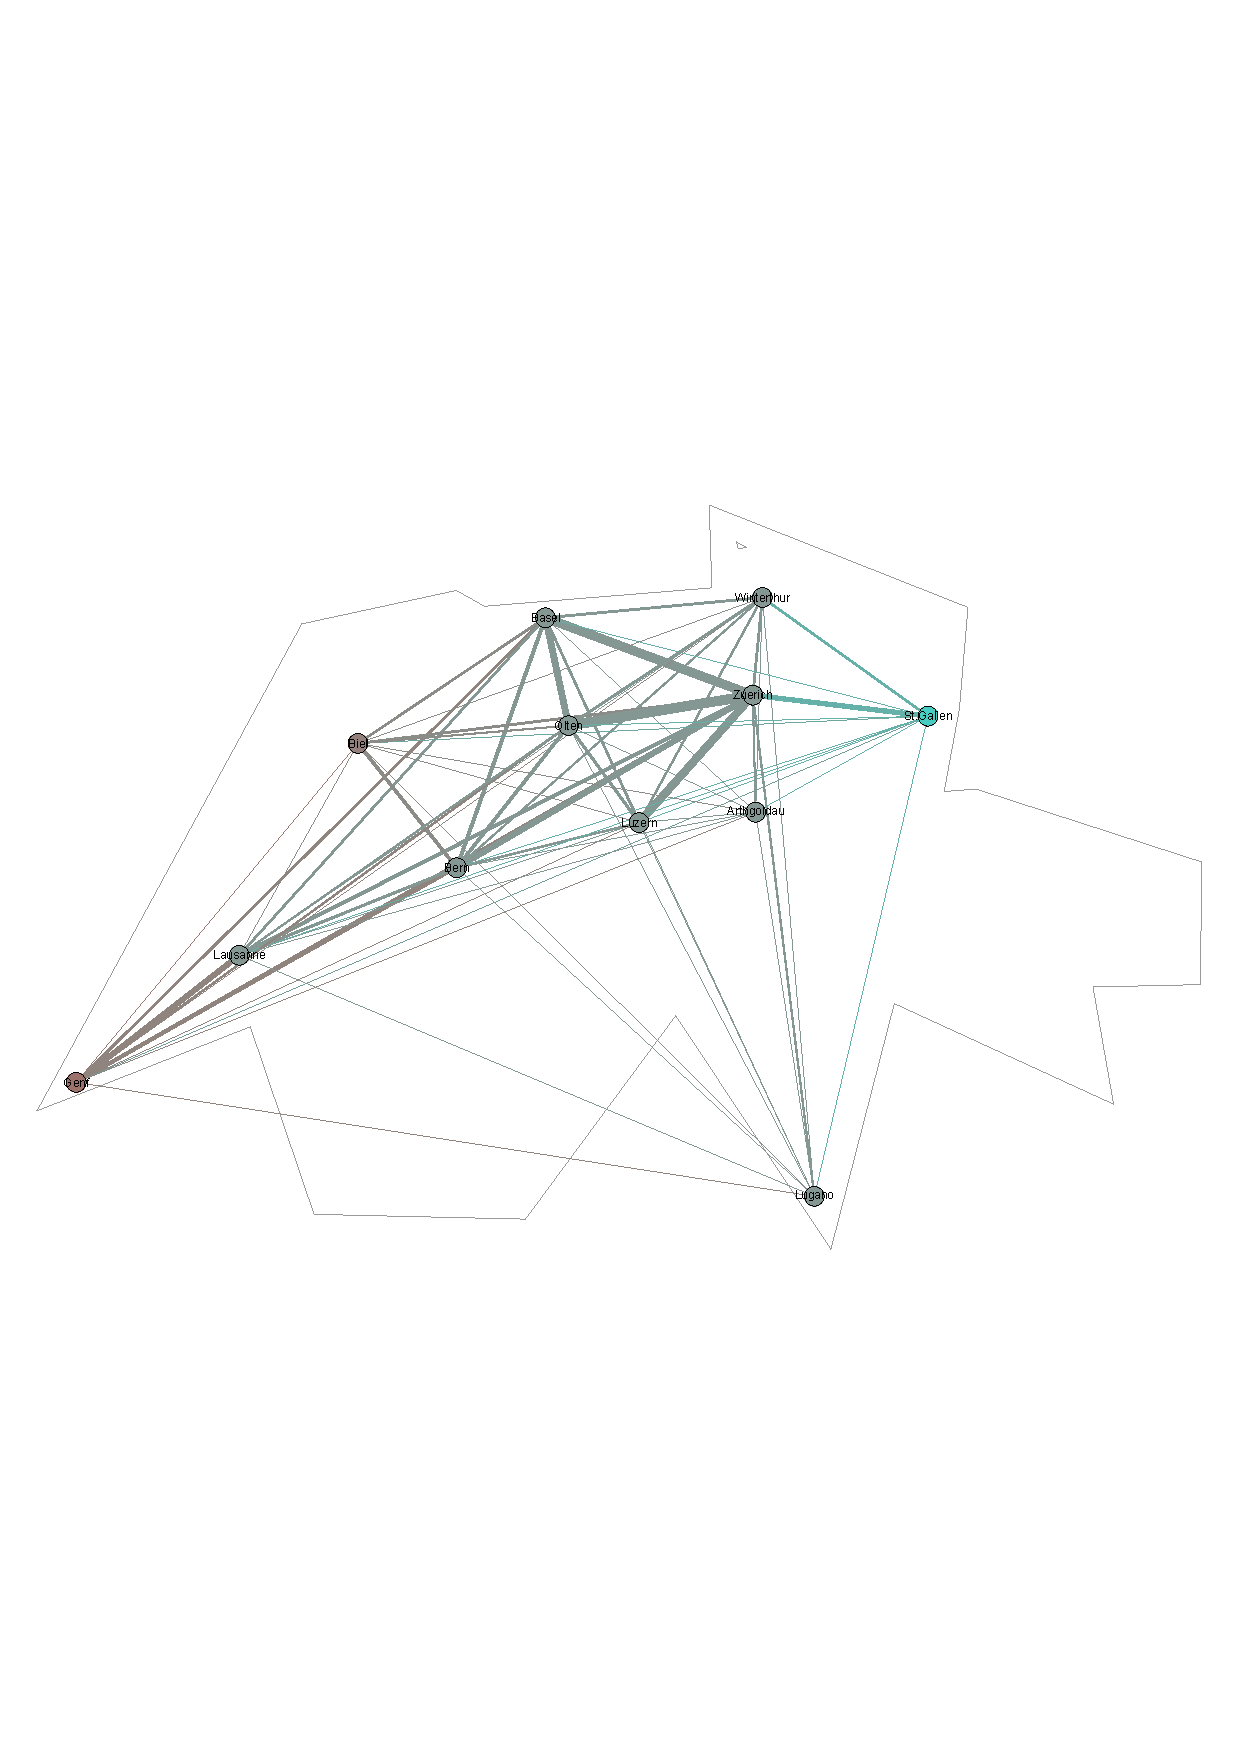
\includegraphics[scale=0.25]{switzerland_network1}
 \caption{Gravity model 1: Model of the 10 biggest cities plus two additional one. Layout by gephi with respection geographical position.}
\end{figure}

!!!!!!!!!!Do eventuell no omschriebe wennn mers so wei schtrukturiere ond e teil is next chapter!!!!!!!!!!!!!!!!!!!!!!!!!!!!!!!!!!!!!!!
This was the first network we plotted. While looking at the picture it was striking that the network didn't at all cover the hole country. Espacially the south-west part was unattended. So we extended the number of cities to 20 and keept the two addtional ones from the beginning.


\subsection{The Extended Connectionmatrix Gravity Model}
In the general gravity model we used geographical distance as the distance indicator. But we thought it would also be reasonable to use the time it takes to travel from one city to the other as the distance indicator. The idea was that this also takes in account if there is obstacle like a mountain or a lake between the cities. A disadvantige of it is, that in a way one approximate the network with the existing network. Anyway we scipted that later because it meant a lot of -unnecessary- work.


\subsection{Investigation of the resulting network(theory of network parameters)}



\section{Implementation}
\textbf{In general we tried to be as specific as possible with the commentation of the funcitons in matlab}

We created a script called data1 which contains all our relevant data.

\subsection{Networkflow-function}
First we implemented a general network function which applys the theory mentioned in the description of the model to an adjacency matrix of a network. This function gave another adjacency matrix back with the simulate flow. This function would also run for every other gravity model based simulation.\newline

For the distance based gravity function we also need the geographical distance. For that purpose we added to each city its coordinates and computed the distance between each city by just applying phythagors. Since Switzerland is a small country we did not taken in account that the earth is a spehre and just approximatied as if it was a plane. The function gives again a adicency matrix back.


\subsection{Visualization}
In the lectures it was recommended to use gephi. So some of our pictures are made with it. But a huge disadvantige of gephi is that it is rather complicated to respect geographical position if one uses an adiacency  matrix to represend the network. In figure 1 we placed the cities by hand.

But since this is rather complicated we also wrote funciton in matlab to illustrate a network given in a adjacency matrix. The result isn't as pretty as in gephi so both methodes have their advantages and disadvantages.

\subsection{Investigation-function}




We formed the distance information into a adjacency matrix to represent the connections between the cities.  We characterised a connection to be only direct. For example if a train goes from ZÃŒrich to Lausanne and stops in Bern, it will be counted as 2 connections (ZÃŒrich-Bern, Bern-Lausanne). The entry in the matrix of a connection is the time .... muesi do so triviale shit schribe???????????




\section{Simulation Results and Discussion}

\section{Summary and Outlook}

\section{References}






\end{document}  